\chapter{Results}
% TODO: Rewrite chapter 4 as results
% 1 - Scalability, fix number of MEC and increase number of UEs
% Show learning, show performance
% 2 - Robustness, change system hyper parameters
% Show leaning and performance
% 3 - Show impact of worst case scenario reward
% Show learning and performance as increasing max weight

\section{Baselines}
\noindent In order to benchmark the various \acrshort{DRL} algorithms and test the implemented simulator, several baseline algorithms were developed:

\begin{itemize}
    \item Full local: all \acrshort{UE}s execute their tasks locally, in terms of the decision vector $\mathcal{A}=[0_1, 0_2, ..., 0_N]$. This represents the case where the system has no offloading capabilities.
    \item Random Offload: where offloading decision is completely random, each task is then executed locally or offloaded to one of the available \acrshort{MEC} servers randomly;
    \item Full nearest \acrshort{MEC}: all \acrshort{UE} tasks are offloaded to the nearest \acrshort{MEC} server according to Equation (\ref{distance_nm}). This represents the case of offloading to the nearest node without regarding their computation constraints and other offloading decisions.
\end{itemize}

To put these baselines and the simulator to the test, a simple test case was devised. In this test, there are five \acrshort{UE}s and five \acrshort{MEC} servers. The UEs and MEC servers were randomly distributed in a 2D plane with $x \in [0, 200]$ and $y \in [0, 200]$, resulting in the distribution seen in Figure \ref{example_layout}.

\begin{figure}[h]
  \centering
  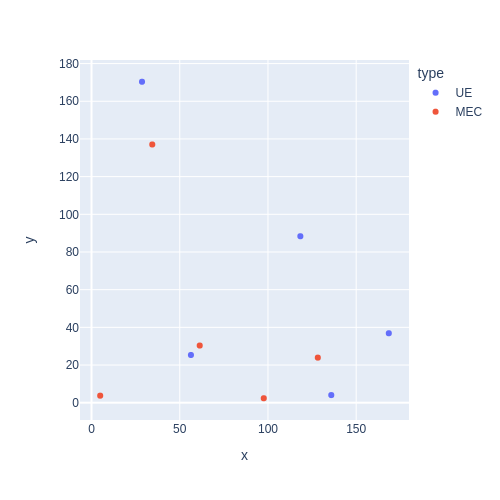
\includegraphics[width=200px]{images/example_layout.png}
  \caption{Example layout for the simple test}  \label{example_layout}
\end{figure}

For simplicity all \acrshort{UE}s and \acrshort{MEC} servers are considered to have the same specifications. The system hyper-parameters were set according to the values present in Table \ref{hyperparams}. In order to test this configuration the task parameters, $B_n$, $B_d$ and $D_n$ were sampled from uniform distributions between ($300$, $500$) Kbits, ($10$, $15$) Kbits and ($900$, $1100$) Megacyles respectivly. Each algorithm ran for 100 iterations and an average cost of offloading decisions is shown in Table \ref{resultstest1}.


% Please add the following required packages to your document preamble:
% \usepackage[normalem]{ulem}
% \useunder{\uline}{\ul}{}
\begin{table}[h]
\centering
\begin{tabular}{|l|l|l|l|}
\hline
Variable             & Value & Variable                & Value \\ \hline
$B$&$10\times10^{6}$&$f_n^l$&$1\times10^{9}$\\
$n$&$10$&$I_n^t$&$0.5$\\
$\beta$&$-4$&$I_n^e$&$0.5$\\
$h_ul$&$100$& $P_m$&$200$\\
$h_dl$&$100$& $P_n$& $500\times10^{-3}$\\
$g_ul$&$1$&$P_n^i$&$100\times10^{-3}$\\
$g_dl$&$1$&$P_n^d$&$200\times10^{-3}$\\
$N_0$&$5\times10^{-5}$&$F_m$&$5\times10^{9}$\\ \hline
\end{tabular}
\caption{System hyper-parameters}\label{hyperparams}
\end{table}

\begin{table}[h]
\centering
\begin{tabular}{|l|l|}
\hline
Algorithm        & Average Cost ($C_{all})$ \\ \hline
Full local       & 13.768\\
Random Offload   & 11.493\\
Full nearest MEC & 1.035\\ \hline
\end{tabular}
\caption{Average Cost ($C_{all}$) over 100 iterations} \label{resultstest1}
\end{table}

The plan is to create several system configurations of increasing complexity. The baseline algorithms will be used in order to benchmark the quality of trained agents. It is expected that the proposed network manager will surpass their performance in all situations by making intelligent decisions taking into account computation, battery, delay and communication constraints ignored by the baselines.